\documentclass{standalone}
\usepackage{graphicx}	
\usepackage{amssymb, amsmath, amsthm}
\usepackage{color}

\usepackage{tikz}
\usetikzlibrary{math, calc}

\definecolor{light}{RGB}{220, 188, 188}
\definecolor{mid}{RGB}{185, 124, 124}
\definecolor{dark}{RGB}{143, 39, 39}
\definecolor{highlight}{RGB}{180, 31, 180}
\definecolor{gray10}{gray}{0.1}
\definecolor{gray20}{gray}{0.2}
\definecolor{gray30}{gray}{0.3}
\definecolor{gray40}{gray}{0.4}
\definecolor{gray60}{gray}{0.6}
\definecolor{gray70}{gray}{0.7}
\definecolor{gray80}{gray}{0.8}
\definecolor{gray90}{gray}{0.9}
\definecolor{gray95}{gray}{0.95}

\begin{document}

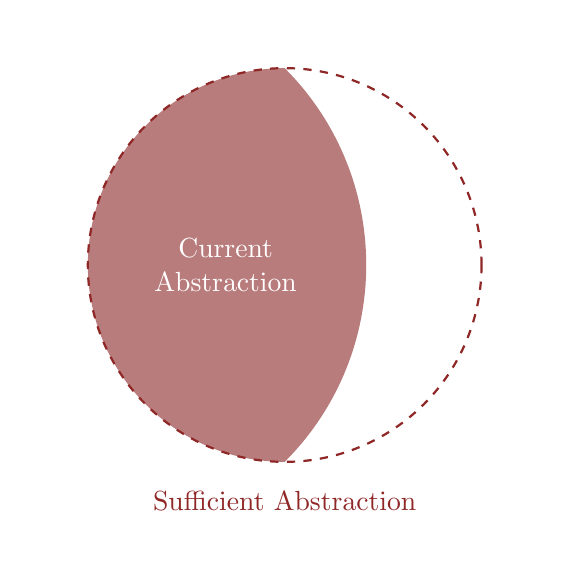
\begin{tikzpicture}[scale=1, thick]
  \draw[white] (-3.25, -3.5) rectangle (3.25, 3);

  %\fill[mid] (-1.5, 0) circle (2);
  %\fill[light] (-3, 0) circle (1.5);
  
  \pgfmathsetmacro{\r}{2.5}
  \pgfmathsetmacro{\theta}{90}
  \pgfmathsetmacro{\delta}{2.5}
  \pgfmathsetmacro{\phi}{atan( \r * sin(\theta) / ( \r * cos(\theta) + \delta) )}
  \pgfmathsetmacro{\R}{sqrt(\r * \r + 2 * \delta * \r * cos(\theta) + \delta * \delta)}

  \fill[mid] ({-\theta}:\r) arc ({-\theta}:{\theta - 360}:\r)
          -- ({\r * cos(\theta)}, {\r * sin(\theta)}) arc ({\phi}:{-\phi}:\R);
  
  \node[white, align=center] at (-0.75, 0) { Current\\Abstraction };

  \draw[dark, dashed] (0, 0) circle (2.5);
  \node[dark] at (0, -3) { Sufficient Abstraction };
  
\end{tikzpicture}

\end{document}  